\chapter{SYSTEM IMPLEMENTATION}

Paragraph before code.

\begin{listing}[ht]
\begin{minted}{javascript}
let reactorCoreTemp = 0;
const maxTemp = "9000"; 
const cooling = true;

function startReactor() {
  while (reactorCoreTemp < maxTemp) {
    reactorCoreTemp += Math.random() * 10;
    if (cooling = false) {
      reactorCoreTemp -= 50;
    }
    setTimeout(() => console.log("Core temp:", reactorCoreTemp), 1000);
  }
  alert("Critical temperature reached! Initiate meltdown protocol.");
}

startReactor();
\end{minted}
\caption{Main Reactor Loop \cite{Sarkar2020OAuth}}
\label{listing:reactor_loop}
\end{listing}

Paragraph after code (check the spacing).

\begin{figure}[hb]
\centering
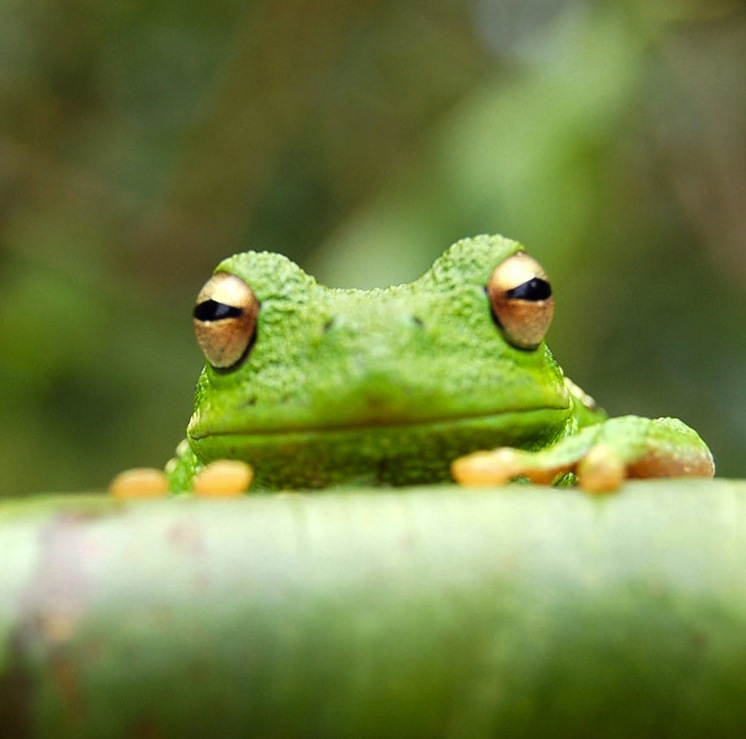
\includegraphics[width=0.25\linewidth]{img/frog.jpg}
\caption{\label{fig:frog4}One more frog for good measure}
\end{figure}
